\section{Analysis}
\label{sec:Analysis}

\subsection{Kinematics of the simulated data}
\label{sec:simdata}
To get to know the $B^{\pm} \to K^{\pm}K^+K^-$ decay, the simulated data is analysed for its kinematic properties. The x, y and z components of the momentum
of one of the hadrons are shown in \autoref{fig:P_H1XYZ}. The momenta in the x- and y- direction follow a gaussian distribution. These two axes are perpendicular
to the beam. However, the z-component shows negative exponential behaviour.
\begin{figure}
  \centering
  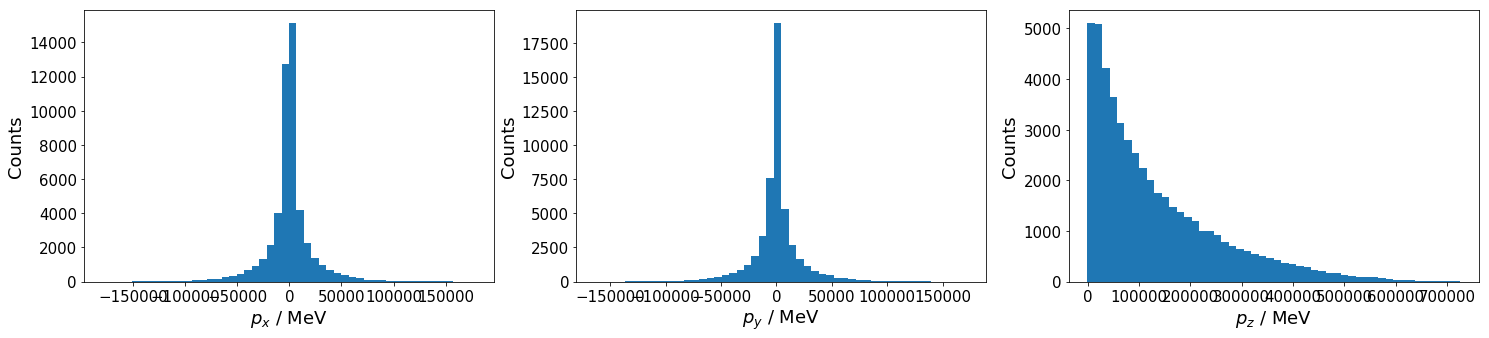
\includegraphics[width = .95\textwidth]{"content/pics/P_H1XYZ.png"}

  \caption{Histograms of the distributions of the momentum vector components for the first hadron of the simulated data.}
  \label{fig:P_H1XYZ}
\end{figure}
\\ With these quantities, the magnitude of the momentum is calculated via 
\begin{equation}
  \label{eq:magn_p}
    p = \sqrt{p_x^2 + p_y^2 + p_z^2}.
\end{equation}
This is done for every kaon candidate and every event.
The resulting distribution of the magnitude of the momentum is shown in \autoref{fig:P_H1}.
\begin{figure}
  \centering
  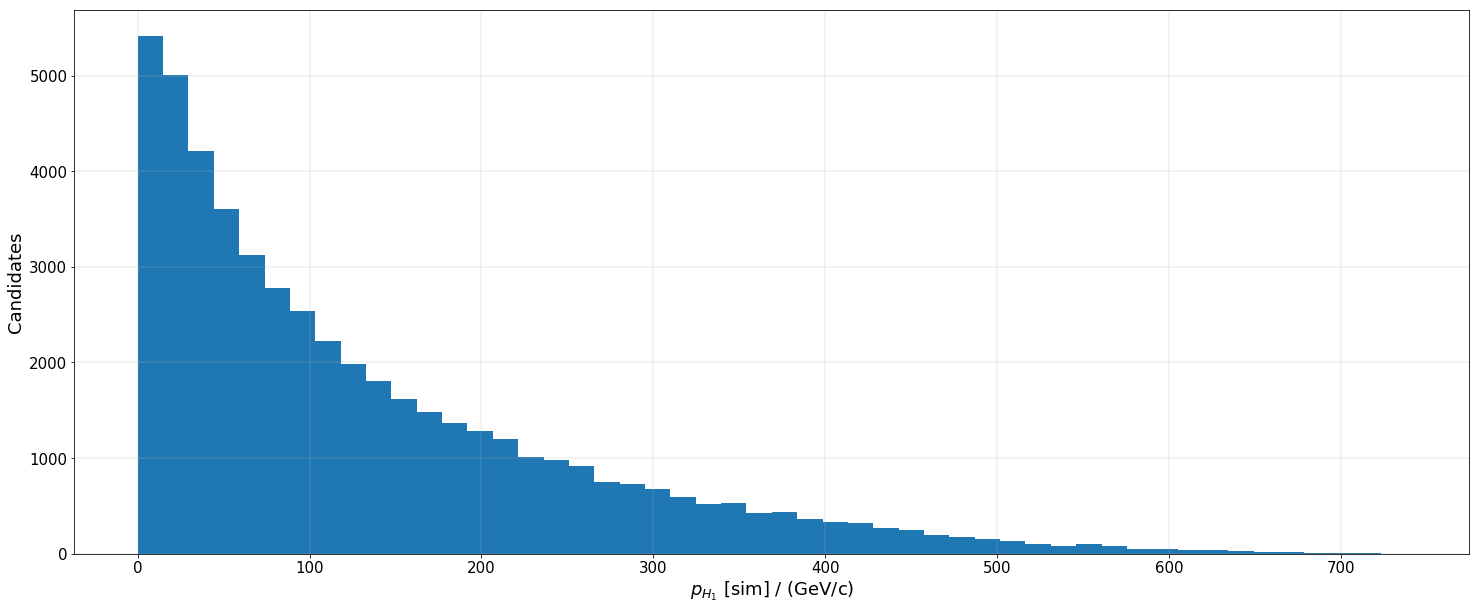
\includegraphics[width = .7\textwidth]{"content/pics/P_H1.png"}
  \caption{Histogram of the magnitude of the momentum for the first hadron of the simulated data.}
  \label{fig:P_H1}
\end{figure}
\\ By using the relation of energy, mass and momentum given by 
\begin{equation}
  \label{eq:energy-momentum-mass}
  E^2 = p^2 + m^2,
\end{equation}
the energy of the hadrons is calculated. The kaon mass is well known and given by $m_{K^{\pm}} = \qty{493.677(0.015)}{\mega\electronvolt}$ \cite{PDG}. The resulting energy distribution of the first hadron is presented in \autoref{fig:E_H1}.
\begin{figure}
  \centering
  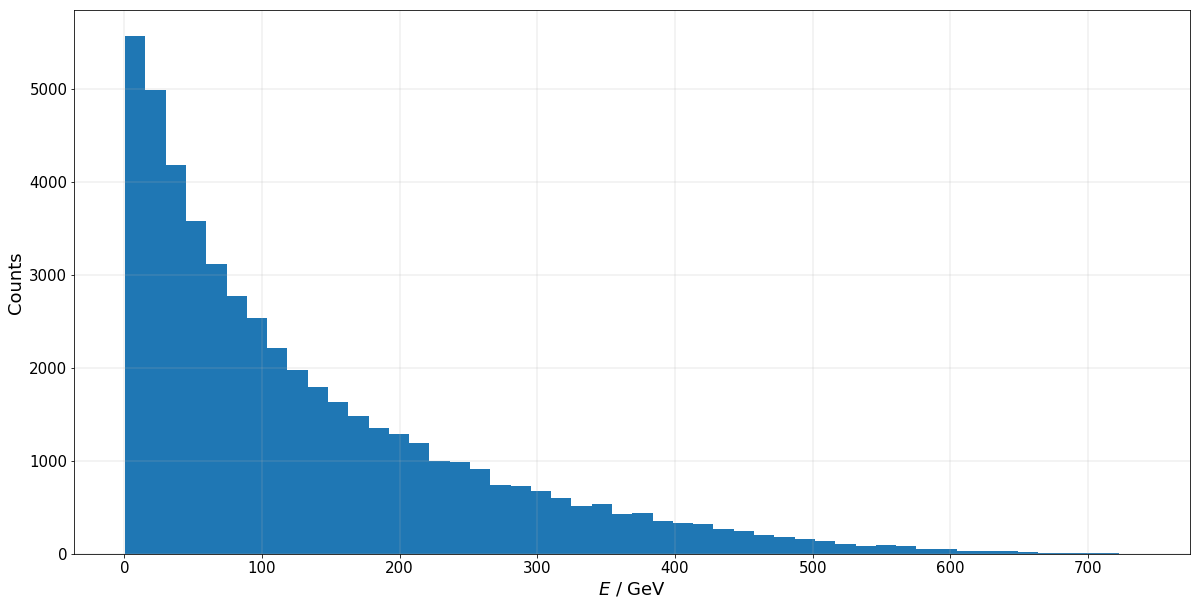
\includegraphics[width = .7\textwidth]{"content/pics/E_H1.png"}
  \caption{Histogram of the energy of the first hadron of the simulated data.}
  \label{fig:E_H1}
\end{figure}
\\The energy is also calculated for the other kaon candidates. Since energy and momentum are conserved quantities, the energy and momentum of the $B^{\pm}$ meson can be calculated
using the energy and momentum of the three kaon candidates. The single momentum components of all final state particles are added together and the magnitude of the momentum of the $B^{\pm}$
meson can be calculated via \autoref{eq:magn_p}. The energy is calculated by summing the energy of all final state particles. With the energy and the magnitude of the momentum, the resulting
mass of the $B^{\pm}$ meson can be calculated via \autoref{eq:energy-momentum-mass}. The resulting distribution can be seen in \autoref{fig:B_M_sim}.
\begin{figure}
  \centering
  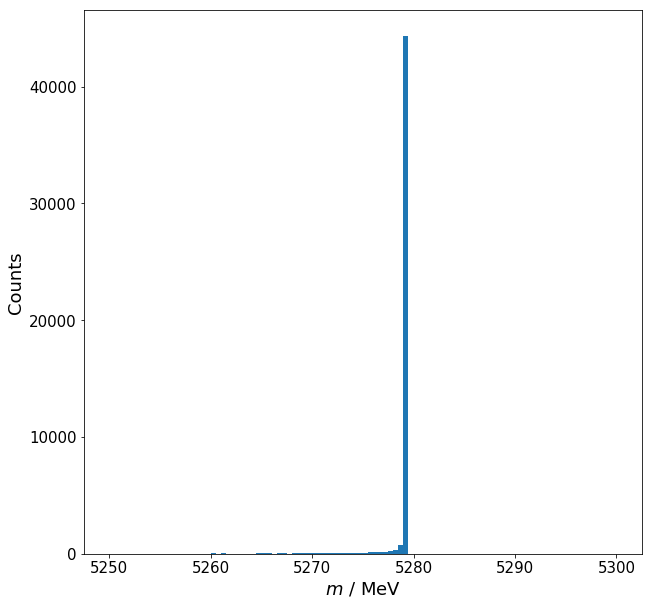
\includegraphics[width = .6\textwidth]{"content/pics/B_M_sim.png"}
  \caption{Histogram of the mass of the $B^{\pm}$ meson of the simulated data.}
  \label{fig:B_M_sim}
\end{figure}
The distribution has a sharp peak at the mass of the $B^{\pm}$ meson ($m_{B^{\pm}} = \qty{5279.41(0.07)}{\mega\electronvolt}$ \cite{PDG}). This is because the data is simulated data using information about the mass of the $B^{\pm}$ meson during
the simulation process. The distribution for real data would be a lot broader and will also contain combinatorial background.

\subsection{Preselection}

To reduce combinatorial background and misidentified decays as well as selecting only the decay into kaons one has to apply cuts on parameters describing the likeliness
of a final state particle being a kaon, pion or muon. Appropriate requirements are selected using the distributions of the likeliness of the particles being kaons or pions 
shown in \autoref{fig:ProbKPi}. This is done for all three final state
hadrons. The cuts are chosen to have a good signal efficiency while also reducing a lot of background. Also, to ensure that the
hadrons are not muons, the variable \texttt{isMuon} is used for the preselection. The chosen cuts are listed
in \autoref{tab:Preselection}.
\begin{table}[h!]
  \centering
    \begin{tabular}{ |p{3cm}||p{3cm}|p{3cm}|p{3cm}|  }
      \hline
      \multicolumn{4}{|c|}{Preselection} \\
      \hline
      Variable & Hadron 1 &Hadron 2 &Hadron 3\\
      \hline
      \texttt{isMuon} (boolean)   & is not &is not&  is not\\
      \texttt{ProbK}&   $> 0.6$  &$> 0.55$   &$> 0.85$\\
      \texttt{ProbPi} & $< 0.3$ & $< 0.3$&  $< 0.3$\\
      \hline   
    \end{tabular}
    \caption{The chosen cuts for the preselection of the recorded data. The values are chosen according to the distributions shown in \autoref{fig:ProbKPi}.}
    \label{tab:Preselection}
\end{table}

\begin{figure}
  \centering
  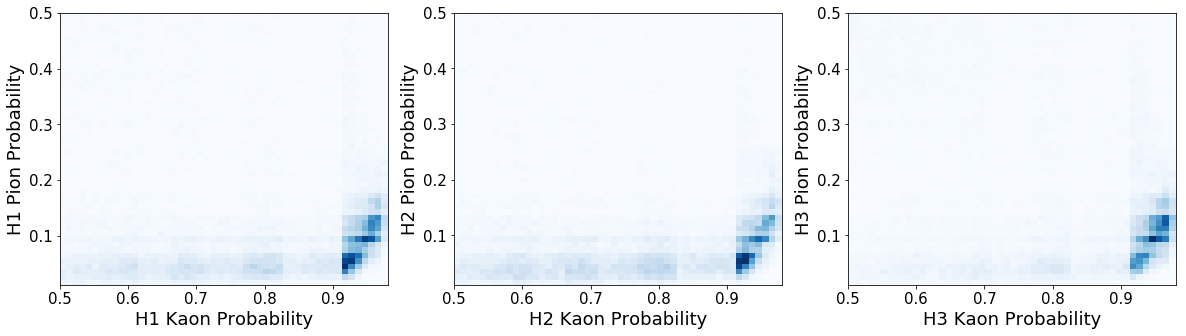
\includegraphics[width = 1\textwidth]{"content/pics/ProbKPi.png"}

  \caption{A 2-dimensional histogram for the Kaon and Pion probability of the three hadrons.}
  \label{fig:ProbKPi}
\end{figure}
The magnitude of the momentum, the energy as well as the mass of the $B^{\pm}$ meson is calculated for the real data, just like it has been done in \autoref{sec:simdata} for the simulated data.
The resulting distribution of the $B^{\pm}$ meson mass can be seen in \autoref{fig:B_M_real}.
\begin{figure}
  \centering
  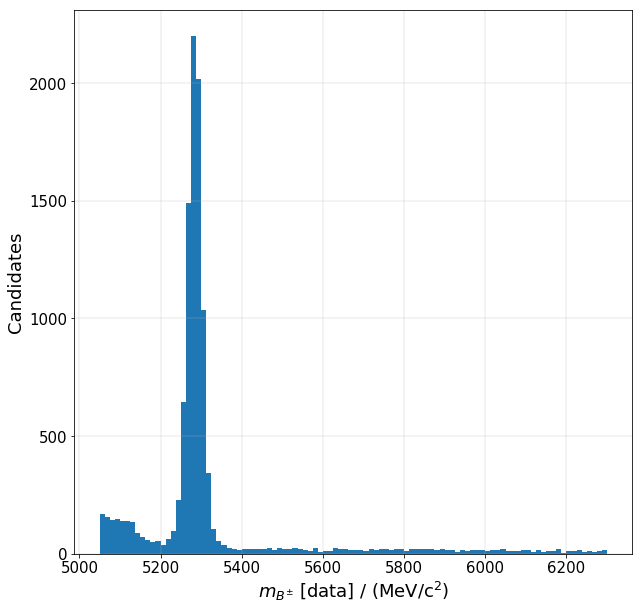
\includegraphics[width = .5\textwidth]{"content/pics/B_M_real.png"}
  \caption{Histogram of the mass of the $B^{\pm}$ meson of the recorded data.}
  \label{fig:B_M_real}
\end{figure}
\\ The gaussian distribution of the mass of the $B^{\pm}$ meson for the recorded data is much broader than the one for the simulated data and also contains uniform background as well as more dominant background on the lower end of the invariant mass.
To reject the background further, a cut on the $B^{\pm}$ meson mass is applied as $m_B > \qty{5230}{\mega\electronvolt}$ and $m_B < \qty{5370}{\mega\electronvolt}$. Multiple 
cuts are tested. The chosen cuts seem to be the best choice for rejected most background, while maintaining much signal.\\

\subsection{Global matter anti-matter differences}

To study possible \textit{CP} violation, the dataset has to be split for events with $B^+ \rightarrow K^+ K^+ K^-$ and $B^- \rightarrow K^- K^+ K^-$. The $B^{\pm}$ meson charge is established by 
looking at the charge of the kaon candidates. Those events, which have two negatively charged kaons came from a $B^-$ meson and those with two positively charged kaons from a $B^+$ meson.
The raw asymmetry is calculated by summing the number of events in each dataset and using \autoref{eq:CP_asymmetry}.\\
The resulting raw global asymmetry for the selected events is $A_{CP,\mathrm{raw}} = 0.0427$. In particle physics, a value is only considered an observation, if it is at least five standard deviations. If it exceeds
three sigma, it is considered evidence. The uncertainty of the asymmetry can be calculated via
\begin{equation}
  \label{eq:unc}
  \sigma_A = \sqrt{\frac{1-A_{CP}^2}{N^+ + N^-}}.
\end{equation}
The significance is the raw asymmetry devided by the resulting uncertainty. The uncertainty for the selected events is $\sigma_{A_{\mathrm{raw}}} = 0.0110$ and the significance is $S_{A_{\mathrm{raw}}} = 3.8803$.
The raw asymmetry is corrected by the underlying production asymmetry arising from the fact, that the particles are
produced by proton-proton collisions. The final asymmetry is calculated by
\begin{equation*}
  A_{CP} = A_{CP,\mathrm{raw}} - A_{CP,\mathrm{prod}}.
\end{equation*}
The production asymmetry is approximated with $1\%$. Therefore, the raw statistical uncertainty is not the only uncertainty that should be considered when analysing decays at LHCb. By using \autoref{eq:unc}, the uncertainty
for the production asymmetry is $\sigma_{A_{prod}} = 0.0110$. Using gaussian error propagation, the global asymmetry, the final uncertainty, and the significance are
\begin{align*}
  A_{CP, \mathrm{global}} &= 0.0327\\
  \sigma_{A_{CP,\mathrm{global}}} &=  0.0156 \\ % \, \, \mathrm{and}\\
  S_{A_{CP,\mathrm{global}}} &= 2.1003.
\end{align*}
The result is therefore no longer considered as evidence for an underlying CP asymmetry.

\subsection{Dalitz plots and resonances}

The decay $B^{\pm} \rightarrow K^{\pm} K^+ K^-$ does not only occur in the direct way, but also with intermediate $R^0$ resonances. These resonances are neutral mesons, which then decay into a pair of positively and negatively
charged kaons. There are two possible combinations for this, since two kaons always have the same charge. To visualise resonances, a Dalitz plot is drawn. For the Dalitz plot, the masses for these two resonance combinations
are calculated just like as for the $B^{\pm}$ meson. The squared masses of the two resonance combinations are then plotted against each other in a two dimensional diagram. It is important to first look up, which kaon candidates are oppositely charged. In this case, the second and third kaon candidate have the same charge. 
Therefore, only the combinations $R_{12}^0$ and $R_{13}^0$ are neutral, with the indices denoting which final state particles are considered. The combination of the second and third particle would mean, that there was a double positively or negatively charged resonance, which is not possible in the Standard Model.
In this plot, resonances are visible by band structures. Depending
on the likeliness of the resonance, these bands can be less or more clear visible.\\
For the simulated data, the Dalitz plot is shown in \autoref{fig:dalitz_sim}. The simulated data does not include resonances and is therefore uniformly distributed.
As for the recorded data, the Dalitz plot is shown in \autoref{fig:dalitz_real}. 
\begin{figure}
  \centering
  \begin{subfigure}[b]{0.45\textwidth}
      \centering
      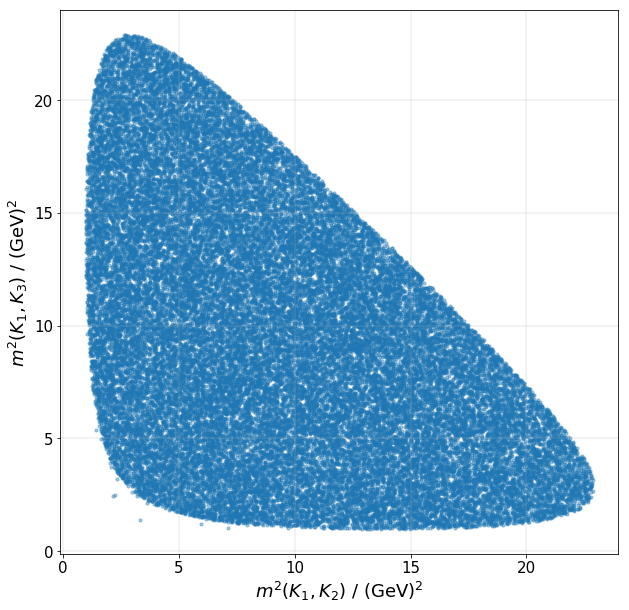
\includegraphics[width=\textwidth]{"content/pics/Dalitz_sim.png"}
      \caption{Dalitz plot of the simulated data.}
      \label{fig:dalitz_sim}
  \end{subfigure}
  \hfill
  \begin{subfigure}[b]{0.45\textwidth}
      \centering
      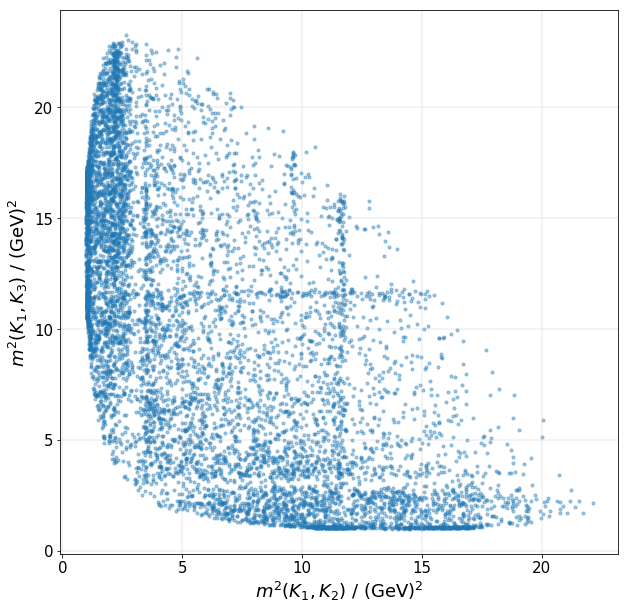
\includegraphics[width=\textwidth]{"content/pics/Dalitz_real.png"}
      \caption{Dalitz plot of the data recorded at the LHCb detector.}
      \label{fig:dalitz_real}
  \end{subfigure}
     \caption{Scatter plots of the Dalitz plots for the simulated data and the recorded data.}
\end{figure}

To make the resonances more visible, it can be helpful to order the resonances $R_{12}$ and $R_{13}$ by mass. This creates a variable "Low", which always includes the resonance with the lower mass and a variable "High" which includes the resonance
with the higher mass. The resulting scatter plot is shown in \autoref{fig:dalitz_real_ordered}. Also, a binned histogram of the data helps to show higher local densities. This is shown in \autoref{fig:dalitz_real_binned}.
\begin{figure}
  \centering
  \begin{subfigure}[b]{0.45\textwidth}
      \centering
      \includegraphics[width=\textwidth]{"content/pics/dalitz_real_ordered.png"}
      \caption{Dalitz plot of the recorded data.}
      \label{fig:dalitz_real_ordered}
  \end{subfigure}
  \hfill
  \begin{subfigure}[b]{0.45\textwidth}
      \centering
      \includegraphics[width=\textwidth]{"content/pics/dalitz_real_ordered_binned.png"}
      \caption{Binned Dalitz plot to visualise local densities.}
      \label{fig:dalitz_real_binned}
  \end{subfigure}
     \caption{Two furter visualisations of the Dalitz plot to make resonances better visual.}
\end{figure}
Especially \autoref{fig:dalitz_real_ordered} shows two main resonances, one being at approximately $\qty{3.5}{} \, \mathrm{\frac{GeV^2}{c^4}}$ and one at approximately $\qty{11.5}{}\, \mathrm{\frac{GeV^2}{c^4}}$. Taking the root of these
values gives the mass of the resonances as $R^0_1 \approx \qty{1870}{}\, \mathrm{\frac{MeV}{c^2}}$ and $R^0_2 \approx \qty{3390}{}\, \mathrm{\frac{MeV}{c^2}}$. The first resonance $R^0_1$ as the $D^0$ meson 
($m_{D^0} = \qty{1864.84(0.05)}{}\, \mathrm{\frac{MeV}{c^2}}$\cite{PDG}) and the second resonance $R^0_2$ as the $\chi_{c0}$ meson ($m_{\chi_{c0}} = \qty{3414.71(0.30)}{}\, \mathrm{\frac{MeV}{c^2}}$\cite{PDG}).

\subsection{Local matter anti-matter differences}

The aim of this analysis is to observe \textit{CP} violation in charmless $B^{\pm}$ meson decays, cutting out both of the resonances is needed, as they include charm quarks. This is done by excluding the mass ranges  
\begin{align*}
  \qty{1830}{}\, - \qty{1890}{}\, \mathrm{\frac{MeV}{c^2}}  \quad \mathrm{and} \quad \qty{3390}{}\, - \qty{3440}{}\, \mathrm{\frac{MeV}{c^2}}
\end{align*}
for both resonances. The Dalitz plot after and before removing the most significant resonances is shown in \autoref{fig:dalitz_real_ordered_nocharm}. No clear band structures are visible anymore.
\begin{figure}
  \centering
  \includegraphics[width = .8\textwidth]{"content/pics/dalitz_real_ordered_no_charm.png"}
  \caption{Dalitz plots before (right) and after (left) removing charm resonances.}
  \label{fig:dalitz_real_ordered_nocharm}
\end{figure}
\\The \textit{CP} asymmetry is evaluated for different kinematic regions now. To do this, the data is splitted for positively and negatively charged $B$ mesons. The binned dalitz plots for each dataset are shown in \autoref{fig:binned_dalitz_no_charm}.
\begin{figure}
  \centering
  \begin{subfigure}[b]{0.45\textwidth}
      \centering
      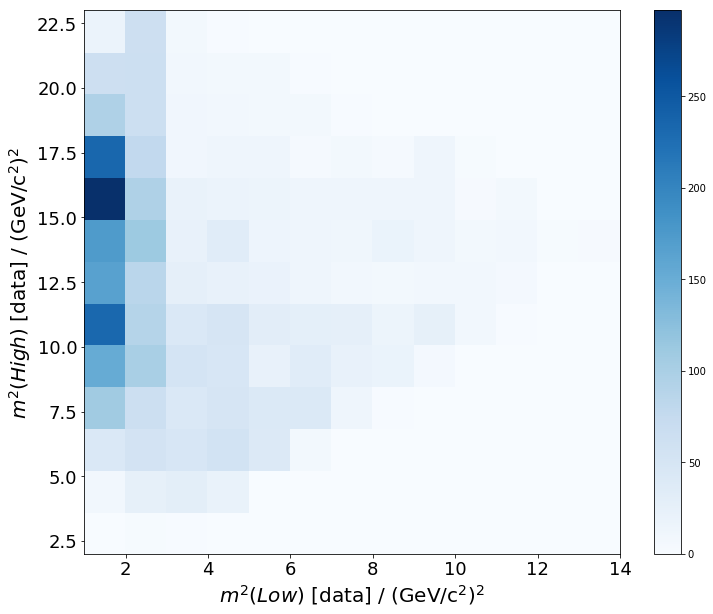
\includegraphics[width=\textwidth]{"content/pics/binned_dalitz_no_charm_p.png"}
      \caption{Binned Dalitz plot of the recorded data including only decays of $B^+$.}
  \end{subfigure}
  \hfill
  \begin{subfigure}[b]{0.45\textwidth}
      \centering
      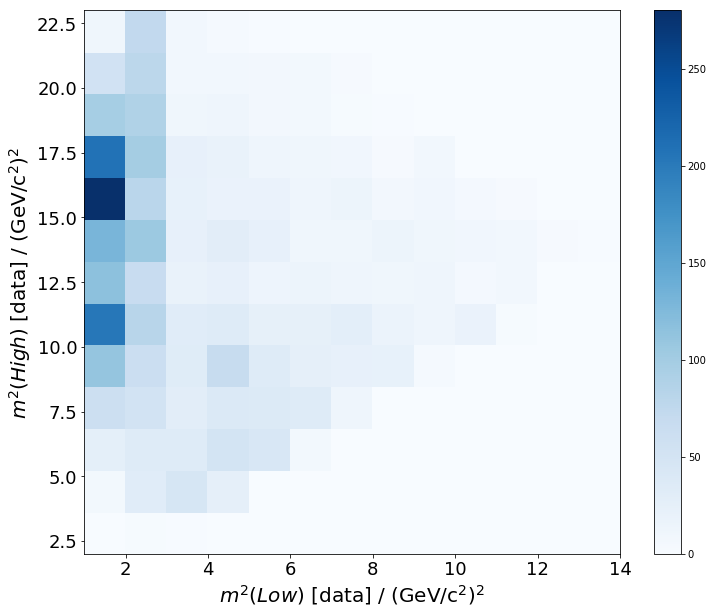
\includegraphics[width=\textwidth]{"content/pics/binned_dalitz_no_charm_m.png"}
      \caption{Binned Dalitz plot of the recorded data including only decays of $B^-$.}
  \end{subfigure}
     \caption{Binned Dalitz plot to visualise local densities.}
     \label{fig:binned_dalitz_no_charm}
\end{figure}
The \textit{CP} asymmetry for each bin is shown in \autoref{fig:binned_asymmetry_no_charm}. 
\begin{figure}
  \centering
  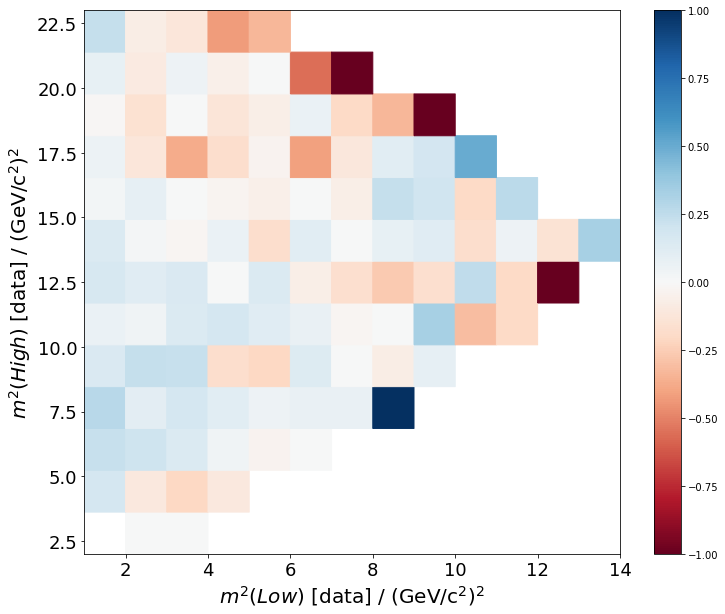
\includegraphics[width = .45\textwidth]{"content/pics/binned_asymmetry_no_charm.png"}
  \caption{Binned \textit{CP} asymmetry for the recorded data.}
  \label{fig:binned_asymmetry_no_charm}
\end{figure}
The resulting \textit{CP} asymmetry can be misleading, if the statistic in the relative bin is too low. To prevent this and extract a meaningful conclusion, the uncertainty and significance per bin is calculated and shown in \autoref{fig:binned_unc_sig_no_charm}.
\begin{figure}
  \centering
  \begin{subfigure}[b]{0.45\textwidth}
      \centering
      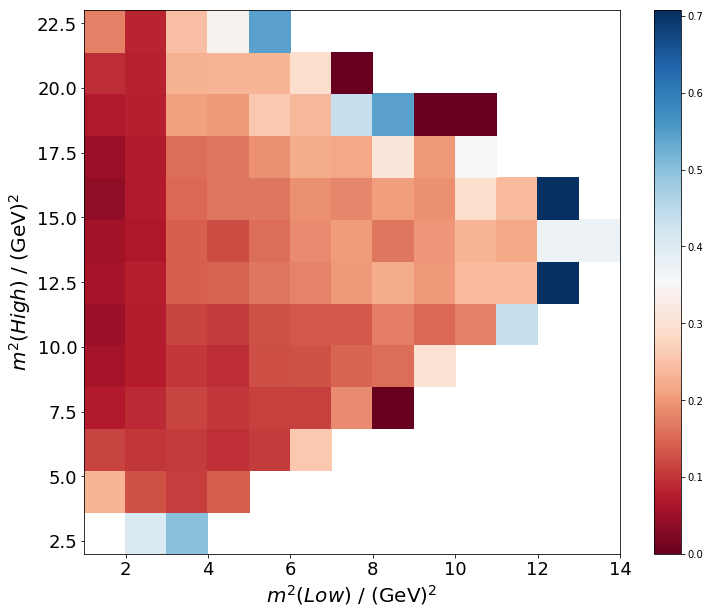
\includegraphics[width=\textwidth]{"content/pics/binned_unc_no_charm.png"}
  \end{subfigure}
  \hfill
  \begin{subfigure}[b]{0.45\textwidth}
      \centering
      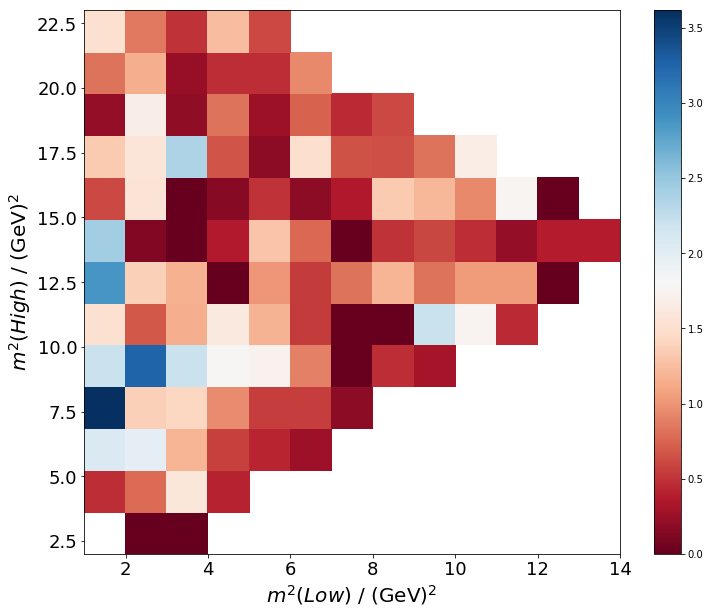
\includegraphics[width=\textwidth]{"content/pics/binned_sig_no_charm.png"}
  \end{subfigure}
     \caption{Binned uncertainty (left) and significance (right) for the caluclated \textit{CP} asymmetry.}
     \label{fig:binned_unc_sig_no_charm}
\end{figure}
As can be seen in \autoref{fig:binned_unc_sig_no_charm} and \autoref{fig:binned_asymmetry_no_charm}, the lower kinematic region shows high significance and asymmetry. This region is extracted by applying a cut as 
\begin{align*}
  m^2_{\mathrm{Low}} < \qty{2}{}\, \mathrm{\frac{GeV^2}{c^4}} \quad \mathrm{and} \quad m^2_{\mathrm{High}}: \qty{6}{} - \qty{10}{}\, \mathrm{\frac{GeV^2}{c^4}} \quad \mathrm{and} \quad \qty{11}{} -  \qty{15}{}\, \mathrm{\frac{GeV^2}{c^4}}
\end{align*}
The mass distribution of the $B^+$ and $B^-$ mesons are shown in \autoref{fig:B_M_after}. 
\begin{figure}
  \centering
    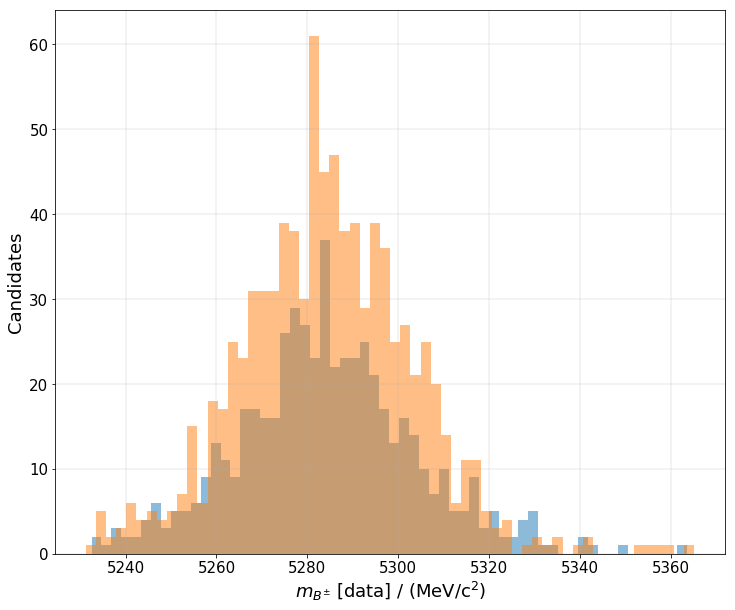
\includegraphics[width=0.5\textwidth]{"content/pics/B_M_real_after_p.png"}
     \caption{Distributions of the invariant mass of the $B^+$ (orange) and $B^-$ (blue) candidates in the relevant bins of the Dalitz plot.}
     \label{fig:B_M_after}
\end{figure}
The resulting local \textit{CP} asymmetry
corrected by the production asymmetry, the overall uncertainty and the significance are
\begin{align*}
  A_{CP,\mathrm{loc}} &= 0.2245\\
  \sigma_{A_{CP,\mathrm{loc}}} &= 0.0282 \\ %\, \, \mathrm{and}\\
  S_{A_{CP,\mathrm{loc}}} &= 7.9628.
\end{align*}
The found local \textit{CP} asymmetry can therefore be called a discovery of a local CP asymmetry in $B^\pm \to K^\pm K^+ K^-$.
